% Options for packages loaded elsewhere
\PassOptionsToPackage{unicode}{hyperref}
\PassOptionsToPackage{hyphens}{url}
%
\documentclass[
]{article}
\usepackage{amsmath,amssymb}
\usepackage{lmodern}
\usepackage{ifxetex,ifluatex}
\ifnum 0\ifxetex 1\fi\ifluatex 1\fi=0 % if pdftex
  \usepackage[T1]{fontenc}
  \usepackage[utf8]{inputenc}
  \usepackage{textcomp} % provide euro and other symbols
\else % if luatex or xetex
  \usepackage{unicode-math}
  \defaultfontfeatures{Scale=MatchLowercase}
  \defaultfontfeatures[\rmfamily]{Ligatures=TeX,Scale=1}
\fi
% Use upquote if available, for straight quotes in verbatim environments
\IfFileExists{upquote.sty}{\usepackage{upquote}}{}
\IfFileExists{microtype.sty}{% use microtype if available
  \usepackage[]{microtype}
  \UseMicrotypeSet[protrusion]{basicmath} % disable protrusion for tt fonts
}{}
\makeatletter
\@ifundefined{KOMAClassName}{% if non-KOMA class
  \IfFileExists{parskip.sty}{%
    \usepackage{parskip}
  }{% else
    \setlength{\parindent}{0pt}
    \setlength{\parskip}{6pt plus 2pt minus 1pt}}
}{% if KOMA class
  \KOMAoptions{parskip=half}}
\makeatother
\usepackage{xcolor}
\IfFileExists{xurl.sty}{\usepackage{xurl}}{} % add URL line breaks if available
\IfFileExists{bookmark.sty}{\usepackage{bookmark}}{\usepackage{hyperref}}
\hypersetup{
  pdftitle={homework4-TK2886},
  hidelinks,
  pdfcreator={LaTeX via pandoc}}
\urlstyle{same} % disable monospaced font for URLs
\usepackage[margin=1in]{geometry}
\usepackage{color}
\usepackage{fancyvrb}
\newcommand{\VerbBar}{|}
\newcommand{\VERB}{\Verb[commandchars=\\\{\}]}
\DefineVerbatimEnvironment{Highlighting}{Verbatim}{commandchars=\\\{\}}
% Add ',fontsize=\small' for more characters per line
\usepackage{framed}
\definecolor{shadecolor}{RGB}{248,248,248}
\newenvironment{Shaded}{\begin{snugshade}}{\end{snugshade}}
\newcommand{\AlertTok}[1]{\textcolor[rgb]{0.94,0.16,0.16}{#1}}
\newcommand{\AnnotationTok}[1]{\textcolor[rgb]{0.56,0.35,0.01}{\textbf{\textit{#1}}}}
\newcommand{\AttributeTok}[1]{\textcolor[rgb]{0.77,0.63,0.00}{#1}}
\newcommand{\BaseNTok}[1]{\textcolor[rgb]{0.00,0.00,0.81}{#1}}
\newcommand{\BuiltInTok}[1]{#1}
\newcommand{\CharTok}[1]{\textcolor[rgb]{0.31,0.60,0.02}{#1}}
\newcommand{\CommentTok}[1]{\textcolor[rgb]{0.56,0.35,0.01}{\textit{#1}}}
\newcommand{\CommentVarTok}[1]{\textcolor[rgb]{0.56,0.35,0.01}{\textbf{\textit{#1}}}}
\newcommand{\ConstantTok}[1]{\textcolor[rgb]{0.00,0.00,0.00}{#1}}
\newcommand{\ControlFlowTok}[1]{\textcolor[rgb]{0.13,0.29,0.53}{\textbf{#1}}}
\newcommand{\DataTypeTok}[1]{\textcolor[rgb]{0.13,0.29,0.53}{#1}}
\newcommand{\DecValTok}[1]{\textcolor[rgb]{0.00,0.00,0.81}{#1}}
\newcommand{\DocumentationTok}[1]{\textcolor[rgb]{0.56,0.35,0.01}{\textbf{\textit{#1}}}}
\newcommand{\ErrorTok}[1]{\textcolor[rgb]{0.64,0.00,0.00}{\textbf{#1}}}
\newcommand{\ExtensionTok}[1]{#1}
\newcommand{\FloatTok}[1]{\textcolor[rgb]{0.00,0.00,0.81}{#1}}
\newcommand{\FunctionTok}[1]{\textcolor[rgb]{0.00,0.00,0.00}{#1}}
\newcommand{\ImportTok}[1]{#1}
\newcommand{\InformationTok}[1]{\textcolor[rgb]{0.56,0.35,0.01}{\textbf{\textit{#1}}}}
\newcommand{\KeywordTok}[1]{\textcolor[rgb]{0.13,0.29,0.53}{\textbf{#1}}}
\newcommand{\NormalTok}[1]{#1}
\newcommand{\OperatorTok}[1]{\textcolor[rgb]{0.81,0.36,0.00}{\textbf{#1}}}
\newcommand{\OtherTok}[1]{\textcolor[rgb]{0.56,0.35,0.01}{#1}}
\newcommand{\PreprocessorTok}[1]{\textcolor[rgb]{0.56,0.35,0.01}{\textit{#1}}}
\newcommand{\RegionMarkerTok}[1]{#1}
\newcommand{\SpecialCharTok}[1]{\textcolor[rgb]{0.00,0.00,0.00}{#1}}
\newcommand{\SpecialStringTok}[1]{\textcolor[rgb]{0.31,0.60,0.02}{#1}}
\newcommand{\StringTok}[1]{\textcolor[rgb]{0.31,0.60,0.02}{#1}}
\newcommand{\VariableTok}[1]{\textcolor[rgb]{0.00,0.00,0.00}{#1}}
\newcommand{\VerbatimStringTok}[1]{\textcolor[rgb]{0.31,0.60,0.02}{#1}}
\newcommand{\WarningTok}[1]{\textcolor[rgb]{0.56,0.35,0.01}{\textbf{\textit{#1}}}}
\usepackage{longtable,booktabs,array}
\usepackage{calc} % for calculating minipage widths
% Correct order of tables after \paragraph or \subparagraph
\usepackage{etoolbox}
\makeatletter
\patchcmd\longtable{\par}{\if@noskipsec\mbox{}\fi\par}{}{}
\makeatother
% Allow footnotes in longtable head/foot
\IfFileExists{footnotehyper.sty}{\usepackage{footnotehyper}}{\usepackage{footnote}}
\makesavenoteenv{longtable}
\usepackage{graphicx}
\makeatletter
\def\maxwidth{\ifdim\Gin@nat@width>\linewidth\linewidth\else\Gin@nat@width\fi}
\def\maxheight{\ifdim\Gin@nat@height>\textheight\textheight\else\Gin@nat@height\fi}
\makeatother
% Scale images if necessary, so that they will not overflow the page
% margins by default, and it is still possible to overwrite the defaults
% using explicit options in \includegraphics[width, height, ...]{}
\setkeys{Gin}{width=\maxwidth,height=\maxheight,keepaspectratio}
% Set default figure placement to htbp
\makeatletter
\def\fps@figure{htbp}
\makeatother
\setlength{\emergencystretch}{3em} % prevent overfull lines
\providecommand{\tightlist}{%
  \setlength{\itemsep}{0pt}\setlength{\parskip}{0pt}}
\setcounter{secnumdepth}{-\maxdimen} % remove section numbering
\ifluatex
  \usepackage{selnolig}  % disable illegal ligatures
\fi

\title{homework4-TK2886}
\author{}
\date{\vspace{-2.5em}}

\begin{document}
\maketitle

\hypertarget{problem-1}{%
\section{Problem 1}\label{problem-1}}

\begin{center}\includegraphics[width=0.5\linewidth]{problem1} \end{center}

\newpage

\hypertarget{problem-2}{%
\section{Problem 2}\label{problem-2}}

\hypertarget{loading-the-crash-data}{%
\subsubsection{Loading the Crash data}\label{loading-the-crash-data}}

\begin{Shaded}
\begin{Highlighting}[]
\NormalTok{crash\_df }\OtherTok{\textless{}{-}} 
  \FunctionTok{read.csv}\NormalTok{(}\StringTok{"Crash.csv"}\NormalTok{)}
\end{Highlighting}
\end{Shaded}

\hypertarget{tidying-the-data}{%
\subsubsection{Tidying the data}\label{tidying-the-data}}

\begin{Shaded}
\begin{Highlighting}[]
\NormalTok{crash\_dfn }\OtherTok{\textless{}{-}}
\NormalTok{  crash\_df }\SpecialCharTok{\%\textgreater{}\%}
  \FunctionTok{pivot\_longer}\NormalTok{(}\FunctionTok{everything}\NormalTok{(), }
               \AttributeTok{names\_to =} \StringTok{"type\_of\_accidents"}\NormalTok{,}
               \AttributeTok{values\_to =} \StringTok{"Values"}\NormalTok{)}
\end{Highlighting}
\end{Shaded}

\hypertarget{problem-2a}{%
\section{Problem 2a}\label{problem-2a}}

\hypertarget{generating-descriptive-statistics-for-each-group}{%
\subsubsection{Generating Descriptive statistics for each
group:}\label{generating-descriptive-statistics-for-each-group}}

\begin{Shaded}
\begin{Highlighting}[]
\NormalTok{crash\_df }\SpecialCharTok{\%\textgreater{}\%} 
  \FunctionTok{summary}\NormalTok{() }\SpecialCharTok{\%\textgreater{}\%} 
\NormalTok{  knitr}\SpecialCharTok{::}\FunctionTok{kable}\NormalTok{(}\AttributeTok{caption =} \StringTok{"Mean, Median, Min, Max, 1st \& 3rd Quartile Values for each type of crash"}\NormalTok{)}
\end{Highlighting}
\end{Shaded}

\begin{longtable}[]{@{}llll@{}}
\caption{Mean, Median, Min, Max, 1st \& 3rd Quartile Values for each
type of crash}\tabularnewline
\toprule
& pedestrian & bicycle & car \\
\midrule
\endfirsthead
\toprule
& pedestrian & bicycle & car \\
\midrule
\endhead
& Min. :29.00 & Min. :28.0 & Min. :20.00 \\
& 1st Qu.:36.00 & 1st Qu.:29.5 & 1st Qu.:21.00 \\
& Median :39.50 & Median :31.5 & Median :22.00 \\
& Mean :37.88 & Mean :32.5 & Mean :23.43 \\
& 3rd Qu.:42.00 & 3rd Qu.:34.5 & 3rd Qu.:24.50 \\
& Max. :43.00 & Max. :39.0 & Max. :31.00 \\
& NA's :2 & NA & NA's :3 \\
\bottomrule
\end{longtable}

\begin{Shaded}
\begin{Highlighting}[]
\NormalTok{crash\_df }\SpecialCharTok{\%\textgreater{}\%} 
  \FunctionTok{summarize\_if}\NormalTok{(is\_numeric, sd, }\AttributeTok{na.rm =}\NormalTok{ T) }\SpecialCharTok{\%\textgreater{}\%}
\NormalTok{  knitr}\SpecialCharTok{::}\FunctionTok{kable}\NormalTok{(}\AttributeTok{caption =} \StringTok{"*Standard deviation* for each type of crash"}\NormalTok{)}
\end{Highlighting}
\end{Shaded}

\begin{longtable}[]{@{}rrr@{}}
\caption{\emph{Standard deviation} for each type of
crash}\tabularnewline
\toprule
pedestrian & bicycle & car \\
\midrule
\endfirsthead
\toprule
pedestrian & bicycle & car \\
\midrule
\endhead
5.43632 & 4.062019 & 3.866831 \\
\bottomrule
\end{longtable}

\begin{Shaded}
\begin{Highlighting}[]
\NormalTok{crash\_dfn }\SpecialCharTok{\%\textgreater{}\%} 
  \FunctionTok{group\_by}\NormalTok{(type\_of\_accidents) }\SpecialCharTok{\%\textgreater{}\%} 
  \FunctionTok{summarise}\NormalTok{(}\AttributeTok{n =} \FunctionTok{n}\NormalTok{(), }\AttributeTok{mean =} \FunctionTok{mean}\NormalTok{(Values, }\AttributeTok{na.rm =}\NormalTok{ T), }
            \AttributeTok{sum =} \FunctionTok{sum}\NormalTok{(Values, }\AttributeTok{na.rm =}\NormalTok{ T), }\AttributeTok{variance =} \FunctionTok{var}\NormalTok{(Values, }\AttributeTok{na.rm =}\NormalTok{ T)) }\SpecialCharTok{\%\textgreater{}\%}
\NormalTok{  knitr}\SpecialCharTok{::}\FunctionTok{kable}\NormalTok{(}\AttributeTok{caption =} \StringTok{"Mean, Variance for each type of crash"}\NormalTok{)}
\end{Highlighting}
\end{Shaded}

\begin{longtable}[]{@{}lrrrr@{}}
\caption{Mean, Variance for each type of crash}\tabularnewline
\toprule
type\_of\_accidents & n & mean & sum & variance \\
\midrule
\endfirsthead
\toprule
type\_of\_accidents & n & mean & sum & variance \\
\midrule
\endhead
bicycle & 10 & 32.50000 & 325 & 16.50000 \\
car & 10 & 23.42857 & 164 & 14.95238 \\
pedestrian & 10 & 37.87500 & 303 & 29.55357 \\
\bottomrule
\end{longtable}

\begin{Shaded}
\begin{Highlighting}[]
\FunctionTok{boxplot}\NormalTok{(Values }\SpecialCharTok{\textasciitilde{}}\NormalTok{ type\_of\_accidents, }\AttributeTok{data =}\NormalTok{ crash\_dfn,}
        \AttributeTok{main =} \StringTok{"Distribution of PTSD score for each type of crash"}\NormalTok{,}
        \AttributeTok{xlab =} \StringTok{"Types of Accident"}\NormalTok{,}
        \AttributeTok{ylab =} \StringTok{"PTSD Score"}\NormalTok{)}
\end{Highlighting}
\end{Shaded}

\includegraphics{HW4-TK2886_files/figure-latex/unnamed-chunk-8-1.pdf}

\hypertarget{analysis-of-differences-observed}{%
\subsubsection{Analysis of Differences
Observed:}\label{analysis-of-differences-observed}}

In the data set that was provided, the mean of the PTSD Score for
Pedestrian Incidents (37.88) is the largest among the three types of
accidents. The mean of the PTSD Score of bicycle incidents (32.50) is
the second highest and the mean of the PTSD Scores for car incidents
(23.43) is the lowest. The standard deviation for PTSD score for
pedestrian incident is 5.44, the standard deviation for PTSD score in
bicycle incident is 4.06, and the standard deviation for the PTSD score
for car crash is 3.87. Pedestrian has a larger standard deviation than
bicycle and car. This indicates that the PTSD score for the pedestrian
incidents is more spread out compared to the other two types if crash.
When pedestrians is involved in an incident, their PTSD score in general
is more varied compared to the other groups (bicycle and cars).
Pedestrian group has the largest standard deviation compared to the
other two groups (bicycle and car) and a large standard deviation
indicates that the data points are far from the mean. The car group has
the smallest standard deviation compared to the other two groups
(pedestrian and bicycle), which indicates that the data points are
clustered closely around the mean.

Furthermore, the boxplot shows that pedestrian and bicycle crash group
has medians over 30, while car crash group has median lower than 30. The
boxplot shows that there is an outlier in the car accident group. Also,
the boxplot for the pedestrian group is somewhat left-skewed, while the
the boxplot for the bicycle and car group is somewhat right-skewed.

\newpage

\hypertarget{problem-2b}{%
\section{Problem 2b:}\label{problem-2b}}

\hypertarget{equations-that-will-be-used-for-problem-2b}{%
\subsubsection{Equations that will be used for problem
2b:}\label{equations-that-will-be-used-for-problem-2b}}

\begin{center}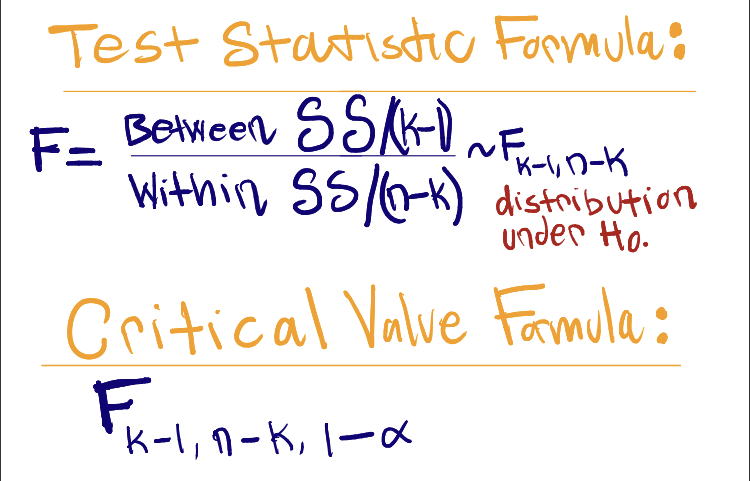
\includegraphics[width=0.5\linewidth]{problem2eq} \end{center}

\hypertarget{assumptions-for-one-way-anova}{%
\subsubsection{Assumptions for One-Way
ANOVA;}\label{assumptions-for-one-way-anova}}

\begin{enumerate}
\def\labelenumi{\arabic{enumi}.}
\item
  There are \emph{k} populations of interest (k\textgreater2): \textbf{k
  = 3}
\item
  The samples are drawn independently from the underlying populations:
\item
  \emph{Homoscedasticity:} the variances of the \emph{k} populations are
  equal;
\item
  \emph{Normality:} the distributions of the error terms are normal:
  \textbf{The problem states it is normally distributed.}
\end{enumerate}

\textbf{The problem does not mention to state the assumptions, but I
asked the professor and the professor emailed me and the professor
stated it is good practice to write the assumptions. Also the problem
does not mention specific things, we assume these assumptions are met to
continue with the test because in problem 2b it states to obtain ``ANOVA
table''.}

\hypertarget{anova-table}{%
\paragraph{ANOVA TABLE}\label{anova-table}}

\begin{Shaded}
\begin{Highlighting}[]
\NormalTok{res1 }\OtherTok{=} \FunctionTok{aov}\NormalTok{(Values }\SpecialCharTok{\textasciitilde{}} \FunctionTok{factor}\NormalTok{(type\_of\_accidents), }\AttributeTok{data =}\NormalTok{ crash\_dfn) }
\FunctionTok{summary}\NormalTok{(res1) }
\end{Highlighting}
\end{Shaded}

\begin{verbatim}
##                           Df Sum Sq Mean Sq F value   Pr(>F)    
## factor(type_of_accidents)  2  790.4   395.2   19.53 1.33e-05 ***
## Residuals                 22  445.1    20.2                     
## ---
## Signif. codes:  0 '***' 0.001 '**' 0.01 '*' 0.05 '.' 0.1 ' ' 1
## 5 observations deleted due to missingness
\end{verbatim}

\begin{Shaded}
\begin{Highlighting}[]
\CommentTok{\# Using R{-}code to obtain critical value }
\NormalTok{critical\_value }\OtherTok{=} \FunctionTok{qf}\NormalTok{(}\FloatTok{0.99}\NormalTok{, }\DecValTok{2}\NormalTok{, }\DecValTok{22}\NormalTok{)}
\end{Highlighting}
\end{Shaded}

\textbf{Interpretation}:

\textbf{Hypothesis:}

\textbf{Ho:} mu1 = mu2 = mu3

\textbf{Ha:} at least two means are not equal

\textbf{Test-Statistics:} F-Value: 19.53 -\textgreater{} \emph{Obtained
from ANOVA table that was created above.}

\textbf{Critical Value:} Critical Value: 5.7190219 -\textgreater{}
\emph{Obtained from R-code above qf().}

\textbf{Interpretation in context to our problem:} Our F-statistics
(19.53) is bigger than our critical value (5.72), we reject the null
hypothesis. At 0.01 significance level, we reject the null hypothesis
and conclude that at least two of true mean PTSD score from the three
type of crash groups are different.

\newpage

\hypertarget{problem-2c}{%
\section{Problem 2c:}\label{problem-2c}}

\begin{Shaded}
\begin{Highlighting}[]
\NormalTok{Tukey\_comp }\OtherTok{=} \FunctionTok{TukeyHSD}\NormalTok{(res1, }\AttributeTok{conf.level =} \FloatTok{0.99}\NormalTok{)}
\NormalTok{Tukey\_comp}
\end{Highlighting}
\end{Shaded}

\begin{verbatim}
##   Tukey multiple comparisons of means
##     99% family-wise confidence level
## 
## Fit: aov(formula = Values ~ factor(type_of_accidents), data = crash_dfn)
## 
## $`factor(type_of_accidents)`
##                         diff        lwr       upr     p adj
## car-bicycle        -9.071429 -16.262165 -1.880692 0.0013441
## pedestrian-bicycle  5.375000  -1.546324 12.296324 0.0492580
## pedestrian-car     14.446429   6.894645 21.998212 0.0000088
\end{verbatim}

\textbf{Analysis:} We will be using be Tukey's adjustment since
Bonferroni is a conservative method and gives us less power while
Tukey's method controls for all pairwise comparisons and it is less
conservative. Based on our Tukey's adjustment method, it is indicated
that the the true mean PTSD score for car and bicycle is different since
the adjusted p-value for car-bicycle pairwise is 0.00134 which is
smaller than our alpha 0.01. Also the the true mean PTSD score for
pedestrian and car is different since the adjusted p-value for
pedestrian-car pairwise is 0.0000088 which is smaller than our alpha
0.01. \emph{Based on the Tukey's method, we do not have enough evidence
to state that the true mean PTSD score for pedestrian-bicycle pairwise
is different}. \emph{It is important to note that in lecture, we did not
go over assumptions for the Tukey and Bonferroni methods. I emailed the
professor and the professor stated that either Tukey or Bonferroni will
be valid to use for this problem.}

\newpage

\begin{Shaded}
\begin{Highlighting}[]
\FunctionTok{plot}\NormalTok{(Tukey\_comp)}
\end{Highlighting}
\end{Shaded}

\includegraphics{HW4-TK2886_files/figure-latex/unnamed-chunk-13-1.pdf}
\textbf{Some reason the code did not output the middle label, it should
be pedestrian-bicycle.} I posted a picture below of what the output
should be with the correct label.

\begin{center}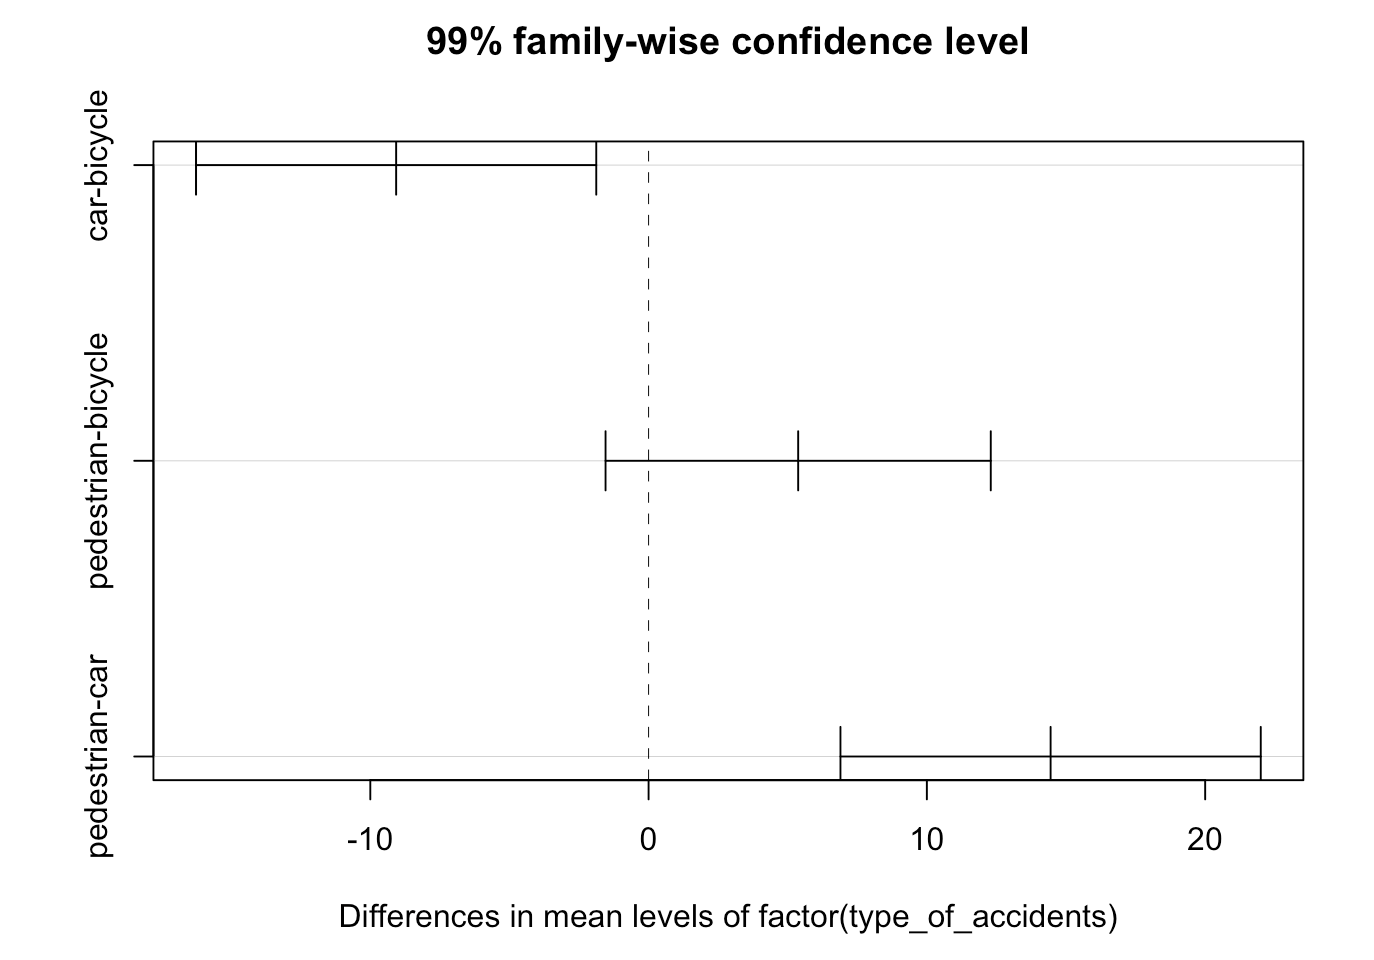
\includegraphics[width=0.5\linewidth]{problem2c} \end{center}

\newpage

\hypertarget{problem-2d}{%
\section{Problem 2d:}\label{problem-2d}}

Based on the data set provided for each type of crash (bicycle, car,
pedestrian), our statistical analysis indicated that the mean PTSD score
for pedestrian is 37.88 and the mean PTSD score bicycle crash is 32.5.
It has been reported by the National Center for PTSD that a PTSD score
of 31-33 or higher suggest the patient may benefit from PTSD treatment.
Emergency Department physicians may provide additional resources or a
better catered treatment plan to individuals involved in pedestrian and
bicycle incidents/crashes for reducing their PTSD symptoms. In our
statistical analysis, the mean PTSD score for car is 23.43 and it has
been reported by the National Center for PTSD that scores lower than
31-33 may indicate the patient either has sub threshold symptoms of PTSD
or does not meet criteria for PTSD. Emergency department physicians
should be aware of which type of crash group on average has higher PTSD
score. Emergency department physicians should give proper or more
medical resources to those groups (which in this case is pedestrian and
bicycle group). Furthermore, our statistical finding indicates that we
do not have enough evidence to state that pedestrian and bicycle mean
for PTSD score are different. In both groups, the calculated mean and
median PTSD score is above 31 and the emergency department physicians
need to provide additional treatment towards these two groups
(pedestrian and bicycle incidents) so that these individuals have less
difficult time in recovering after being involved in or experiencing a
terrifying crash.

\newpage

\hypertarget{problem-3a}{%
\section{Problem 3a:}\label{problem-3a}}

The appropriate test I used to address this question of interest is
\textbf{Chi-Squared of Independence}. Our observational units are
collected at random from a population, we are not gathering the data by
randomly sampling from each sub-group separately, which is the case of
Chi-Squared Test for Homogeneity. Also, we have two categorical
variables (relapse and non-relapse) that are being observed for each
unit (desipramine users, lithium users, and placebo users). We're
interested in whether the knowledge of one variable (type of
antidepressants drug) value provides an information about the value of
the other variable (relapse status), i.e.~are these two variables
independent. Chi-Squared of Homogeneity assesses whether the pattern of
relapse was different between the three groups of antidepressants.

\hypertarget{equations-that-will-be-used-for-problem-3}{%
\subsubsection{Equations that will be used for problem
3:}\label{equations-that-will-be-used-for-problem-3}}

\hypertarget{under-the-null-hypothesis}{%
\paragraph{Under the null hypothesis:}\label{under-the-null-hypothesis}}

\begin{center}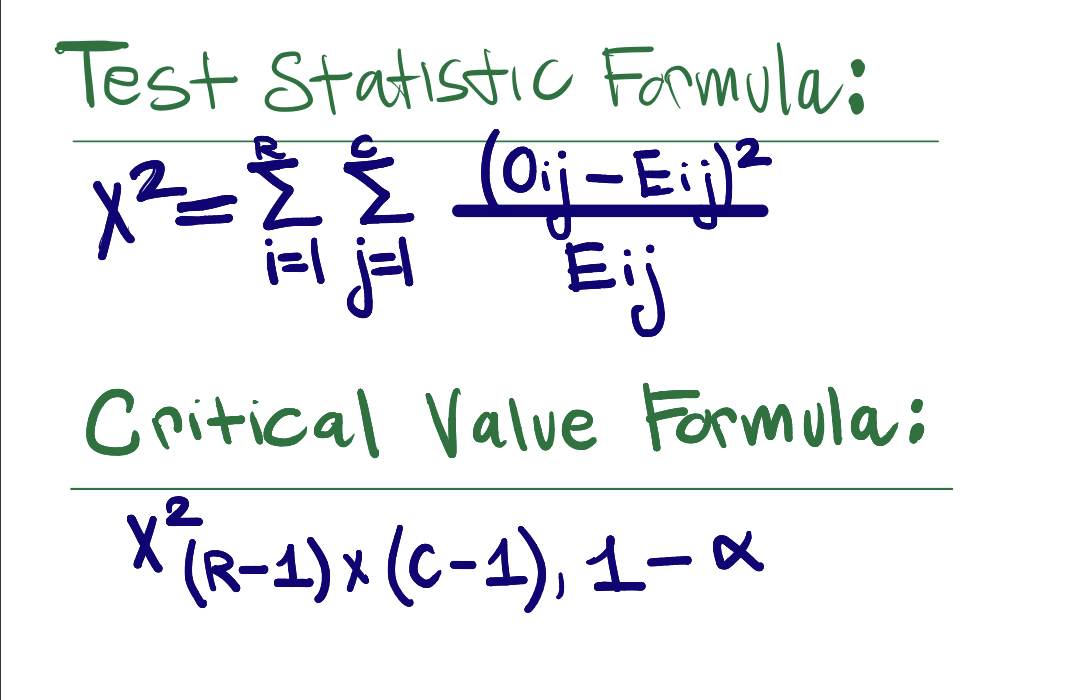
\includegraphics[width=0.5\linewidth]{problem3eq} \end{center}

\textbf{We do not need to use Yates' Continuity Correction, since that
correction is only for 2x2 tables.}

\textbf{Assumptions for Chi-Squared}:

\begin{enumerate}
\def\labelenumi{\arabic{enumi}.}
\item
  Independent Random Sample: Question states ``randomly assigned''
\item
  No expected cell counts are 0, and no more than 20\% of the cells have
  an expected count less than 5: \emph{After creating the table, there
  is no cells with values of 0 and there is no cells with values less
  than 5.}
\end{enumerate}

\newpage

Problem 3b:

\hypertarget{chi-squared-test-of-independence-table}{%
\subsubsection{Chi-Squared: Test of Independence
Table}\label{chi-squared-test-of-independence-table}}

\begin{center}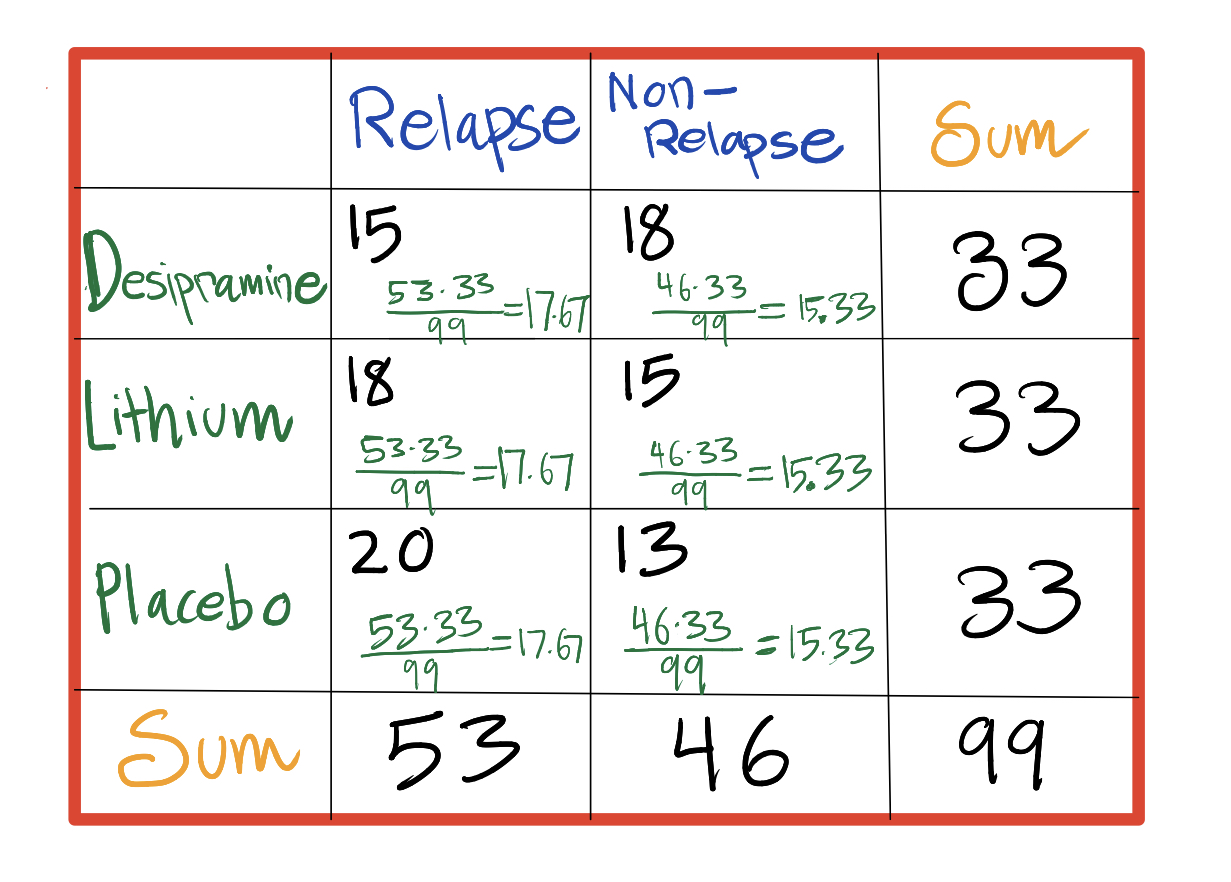
\includegraphics[width=0.5\linewidth]{problem3} \end{center}

\hypertarget{we-may-use-r-code-to-get-the-chi-squared-test-of-independence-table}{%
\subsubsection{We may use R-code to get the Chi-Squared: Test of
Independence
Table}\label{we-may-use-r-code-to-get-the-chi-squared-test-of-independence-table}}

\begin{Shaded}
\begin{Highlighting}[]
\NormalTok{antidepressant\_df }\OtherTok{=} \FunctionTok{matrix}\NormalTok{(}\FunctionTok{c}\NormalTok{(}\DecValTok{15}\NormalTok{, }\DecValTok{18}\NormalTok{, }\DecValTok{18}\NormalTok{, }\DecValTok{15}\NormalTok{, }\DecValTok{20}\NormalTok{, }\DecValTok{13}\NormalTok{), }\AttributeTok{nrow=}\DecValTok{3}\NormalTok{,}\AttributeTok{ncol=}\DecValTok{2}\NormalTok{,}\AttributeTok{byrow=}\NormalTok{T,}
                  \AttributeTok{dimnames =} \FunctionTok{list}\NormalTok{(}\FunctionTok{c}\NormalTok{(}\StringTok{"Desipramine"}\NormalTok{,}\StringTok{"Lithium"}\NormalTok{,}\StringTok{"Placebo"}\NormalTok{), }
                                  \FunctionTok{c}\NormalTok{(}\StringTok{"Relapse"}\NormalTok{,}\StringTok{"Non{-}Relpase"}\NormalTok{)))}

\NormalTok{antidepressant\_dfa }\OtherTok{=} \FunctionTok{addmargins}\NormalTok{(antidepressant\_df)}
\NormalTok{antidepressant\_dfa }\SpecialCharTok{\%\textgreater{}\%}\NormalTok{ knitr}\SpecialCharTok{::}\FunctionTok{kable}\NormalTok{()}
\end{Highlighting}
\end{Shaded}

\begin{longtable}[]{@{}lrrr@{}}
\toprule
& Relapse & Non-Relpase & Sum \\
\midrule
\endhead
Desipramine & 15 & 18 & 33 \\
Lithium & 18 & 15 & 33 \\
Placebo & 20 & 13 & 33 \\
Sum & 53 & 46 & 99 \\
\bottomrule
\end{longtable}

\newpage

\hypertarget{problem-3c}{%
\section{Problem 3c:}\label{problem-3c}}

\begin{Shaded}
\begin{Highlighting}[]
\CommentTok{\#Using R code to get test{-}statistics, p{-}value, degrees od freedom}
\NormalTok{new\_var }\OtherTok{=} \FunctionTok{chisq.test}\NormalTok{(antidepressant\_df)}
\NormalTok{new\_var}
\end{Highlighting}
\end{Shaded}

\begin{verbatim}
## 
##  Pearson's Chi-squared test
## 
## data:  antidepressant_df
## X-squared = 1.5431, df = 2, p-value = 0.4623
\end{verbatim}

\begin{Shaded}
\begin{Highlighting}[]
\NormalTok{new\_var}\SpecialCharTok{$}\NormalTok{expected }\SpecialCharTok{\%\textgreater{}\%}\NormalTok{ knitr}\SpecialCharTok{::}\FunctionTok{kable}\NormalTok{()}
\end{Highlighting}
\end{Shaded}

\begin{longtable}[]{@{}lrr@{}}
\toprule
& Relapse & Non-Relpase \\
\midrule
\endhead
Desipramine & 17.66667 & 15.33333 \\
Lithium & 17.66667 & 15.33333 \\
Placebo & 17.66667 & 15.33333 \\
\bottomrule
\end{longtable}

\begin{Shaded}
\begin{Highlighting}[]
\CommentTok{\#Test Statistics }
\NormalTok{test\_statistic }\OtherTok{=}\NormalTok{ (}\DecValTok{15}\FloatTok{{-}17.67}\NormalTok{)}\SpecialCharTok{\^{}}\DecValTok{2}\SpecialCharTok{/}\FloatTok{17.67} \SpecialCharTok{+} 
\NormalTok{  (}\DecValTok{18}\FloatTok{{-}17.67}\NormalTok{)}\SpecialCharTok{\^{}}\DecValTok{2}\SpecialCharTok{/}\FloatTok{17.67} \SpecialCharTok{+}\NormalTok{ (}\DecValTok{20}\FloatTok{{-}17.67}\NormalTok{)}\SpecialCharTok{\^{}}\DecValTok{2}\SpecialCharTok{/}\FloatTok{17.67} \SpecialCharTok{+} 
\NormalTok{  (}\DecValTok{18}\FloatTok{{-}15.33}\NormalTok{)}\SpecialCharTok{\^{}}\DecValTok{2}\SpecialCharTok{/}\FloatTok{15.33} \SpecialCharTok{+}\NormalTok{ (}\DecValTok{15}\FloatTok{{-}15.33}\NormalTok{)}\SpecialCharTok{\^{}}\DecValTok{2}\SpecialCharTok{/}\FloatTok{15.33} \SpecialCharTok{+}\NormalTok{ (}\DecValTok{13}\FloatTok{{-}15.33}\NormalTok{)}\SpecialCharTok{\^{}}\DecValTok{2}\SpecialCharTok{/}\FloatTok{15.33}
\end{Highlighting}
\end{Shaded}

\begin{Shaded}
\begin{Highlighting}[]
\CommentTok{\#Critical Value }
\NormalTok{critical\_value }\OtherTok{=} \FunctionTok{qchisq}\NormalTok{(.}\DecValTok{95}\NormalTok{, }\DecValTok{2}\NormalTok{)}
\end{Highlighting}
\end{Shaded}

\begin{Shaded}
\begin{Highlighting}[]
\CommentTok{\#p{-}value}
\NormalTok{pval }\OtherTok{=} \FunctionTok{pchisq}\NormalTok{(test\_statistic, }\DecValTok{2}\NormalTok{, }\AttributeTok{lower.tail =} \ConstantTok{FALSE}\NormalTok{)}
\end{Highlighting}
\end{Shaded}

\emph{Hypotheses:}

\textbf{Ho:} Relapse and the type of anti-depressant drug are
independent (p1=p2=p3)

\textbf{Ha:} Relapse and the type of anti-depressant drug are
associated/dependent

\textbf{Test Statistics:} The test statistic is: 1.5431165

\textbf{Critical Value:} The critical value is: 5.9914645

\textbf{P-Value:} The p-value is: 0.4622921

\textbf{Interpretation in context to our problem:} At 0.05 significance
level, we fail to reject the null hypothesis because the Chi-squared
test statistic value is smaller than our critical value (test statistics
\textless{} critical value). We conclude that we do not have enough
evidence that the subject's relapse is associated with the
antidepressant drug the subject was assigned to.

\end{document}
